Գիառոն, Կուբալեն և Մալաֆիյսկին ցույց են տվել, որ $def(K_{2n+1})=n$, $n\in \mathbb{N}$: 3.2 պարագրաֆում հաստատվել է Բորովիցկա-Օլշեվսկայի, Դրգաշ-Բուրչարդտի և Հալուշչակի հիպոթեզը\footnote{M. Borowiecka-Olszewska, E. Drgas-Burchardt, M. Ha\l uszczak, On the structure and deficiency of $k$-trees with bounded degree, Discrete Appl. Math. 201, 2016, pp. 24-37.}, համաձայն որի $def(K_{2n+1}-e)=n-1$: Նաև ցույց է տրվել, որ $w_{def}(K_{2n+1}-e)=3n-1$, $n \in \mathbb{N}$:
\begin{hide}
\begin{theorem}
\label{t3_def_near_complete} Եթե $n\in \mathbb{N}$, ապա $def(K_{2n+1}-e)=n-1$:
\end{theorem}
\begin{proof}[Ապացույց]
Հետևանք \ref{c3_def_complete_minus_edges}-ից ունենք, որ $def(K_{2n+1}-e)\geq n-1$ կամայական $n\in \mathbb{N}$ թվի համար: Ապացույցի համար բավարար է կառուցել $K_{2n+1}-e$-ի $\beta$ ճիշտ կողային ներկում, որի դեֆիցիտը կլինի $def(K_{2n+1}-e,\beta)=n-1$: Դիցուք
$V(K_{2n+1}-e)=\left\{v_{0},v_{1},\ldots,v_{2n}\right\}$: Առանց ընդհանրությունը խախտելու կարող ենք ենթադրել, որ $e=v_{1}v_{2n}$:

Սահմանենք $K_{2n+1}-e$-ի $\beta$ կողային ներկումը: Կամայական
$v_{i}v_{j}\in E(K_{2n+1})$ կողի համար, որտեղ $i<j$ և $(i,j)\neq (1,2n)$,
$\beta\left(v_{i}v_{j}\right)$ գույնը որոշենք հետևյալ կերպ.\\

$\beta\left(v_{i}v_{j}\right)=\left\{
\begin{tabular}{ll}
$1$, & երբ $i=0$, $j=1$,\\
$2n+1$, & երբ $i=0$, $j=2$,\\
$j-1$, & երբ $i=0$, $3\leq j\leq n$,\\
$n+1+j$, & երբ $i=0$, $n+1\leq j\leq 2n-2$,\\
$n$, & երբ $i=0$, $j=2n-1$,\\
$2n$, & երբ $i=0$, $j=2n$,\\
$i+j-1$, & երբ $1\leq i\leq \left\lfloor\frac{n}{2}\right\rfloor$,
$2\leq j\leq n$, $i+j\leq n+1$,\\
$i+j+n-2$, & երբ $2\leq i\leq n-1$, $\left\lfloor
\frac{n}{2}\right\rfloor +2\leq j\leq n$, $i+j\geq n+2$,\\
$n+1+j-i$, & երբ $3\leq i\leq n$, $n+1\leq j\leq 2n-2$, $j-i\leq
n-2$,\\
$j-i+1$, & երբ $1\leq i\leq n$, $n+1\leq j\leq 2n$, $j-i\geq n$,\\
$2i-1$, & երբ $2\leq i\leq 1+\left\lfloor
\frac{n-1}{2}\right\rfloor$, $n+1\leq j\leq n+\left\lfloor
\frac{n-1}{2}\right\rfloor$, $j-i=n-1$,\\
$i+j-1$, & երբ $\left\lfloor \frac{n-1}{2}\right\rfloor +2\leq i\leq
n$, $n+1+\left\lfloor \frac{n-1}{2}\right\rfloor\leq j\leq 2n-1$,
$j-i=n-1$,\\
$i+j-2n+1$, & երբ $n+1\leq i\leq n+\left\lfloor
\frac{n}{2}\right\rfloor -1$, $n+2\leq j\leq 2n-2$, $i+j\leq
3n-1$,\\
$i+j-n$, & երբ $n+1\leq i\leq 2n-1$, $n+\left\lfloor
\frac{n}{2}\right\rfloor +1\leq j\leq 2n$, $i+j\geq 3n$:
\end{tabular}%
\right.$\\

Ապացուցենք, որ $\beta$-ն $K_{2n+1}-e$-ի ճիշտ ներկում է $(3n-1)$ գույներով և $def(K_{2n+1}-e,\beta)=n-1$ դեֆիցիտով:

Դիցուք $G$-ն $K_{2n+1}-e$-ի ենթագրաֆն է ծնված 
$\{v_{1},\ldots,v_{2n}\}$ գագաթներով: Պարզ է, որ $G$-ն իզոմորֆ է $K_{2n}-e$ գրաֆին:
$K_{2n+1}-e$-ի այս $\beta$ ներկումը հիմնված է Թեորեմ \ref{tPetrosyan3n2}-ում կառուցված $K_{2n}$-ի միջակայքային $(3n-2)$-ներկման վրա (այդ ներկումը նկարագրված է \cite{Petrosyan2010} աշխատանքի Թեորեմ 4-ի ապացույցում): % սա առաջին գլխում կա
Վերցնում ենք $K_{2n}$-ի այս միջակայքային $(3n-2)$-ներկումը և $G$-ի բոլոր կողերի գույները շեղում ենք մեկով: Դիցուք $\alpha$-ն $G$-ի ստացված ներկումն է: Օգտվելով այս ներկման հատկությունից, որը նկարագրված է \cite{Petrosyan2010}-ի Հետևանք 6-ում, ստանում ենք % ????

\begin{description}
\item[1)] $S\left(v_{1},\alpha\right)=[2,2n-1]$ և $S\left(v_{2},\alpha\right)=[2,2n]$,

\item[2)] $S\left(v_{i},\alpha\right)=S\left(v_{n+i-2},\alpha\right)=[i,2n-2+i]$ երբ $3\leq i\leq n$,

\item[3)]
$S\left(v_{2n-1},\alpha\right)=[n+1,3n-1]$ և
$S\left(v_{2n},\alpha\right)=[n+1,3n-1]\setminus\{2n\}$:
\end{description}

Այժմ, ըստ $\beta$-ի սահմանման, ունենք

\begin{description}
\item[1)] $S\left(v_{0},\beta\right)=[1,n]\cup [2n,3n-1]$,

\item[2)] $S\left(v_{1},\beta\right)=[1,2n-1]$ և $S\left(v_{2},\beta\right)=[2,2n+1]$,

\item[3)] $S\left(v_{i},\beta\right)=[i-1,2n-2+i]$ և $S\left(v_{n+i-2},\beta\right)=[i,2n-1+i]$ երբ $3\leq i\leq n$,

\item[4)]
$S\left(v_{2n-1},\beta\right)=[n,3n-1]$ և
$S\left(v_{2n},\beta\right)=[n+1,3n-1]$:
\end{description}

Սա ցույց է տալիս, որ $\beta$-ն $K_{2n+1}-e$ գրաֆի ճիշտ կողային ներկում է $(3n-1)$ գույներով և $def(K_{2n+1}-e,\beta)=n-1$ դեֆիցիտով: Ուստի,
$def(K_{2n+1}-e)=n-1$ (Նկ. \ref{K7-minus-edge}):
\end{proof}

\begin{figure}
  \begin{center}
    % \tikzset{near start abs/.style={pos=1cm}}
    % \tikzset{near end abs/.style={pos=-1cm}}
  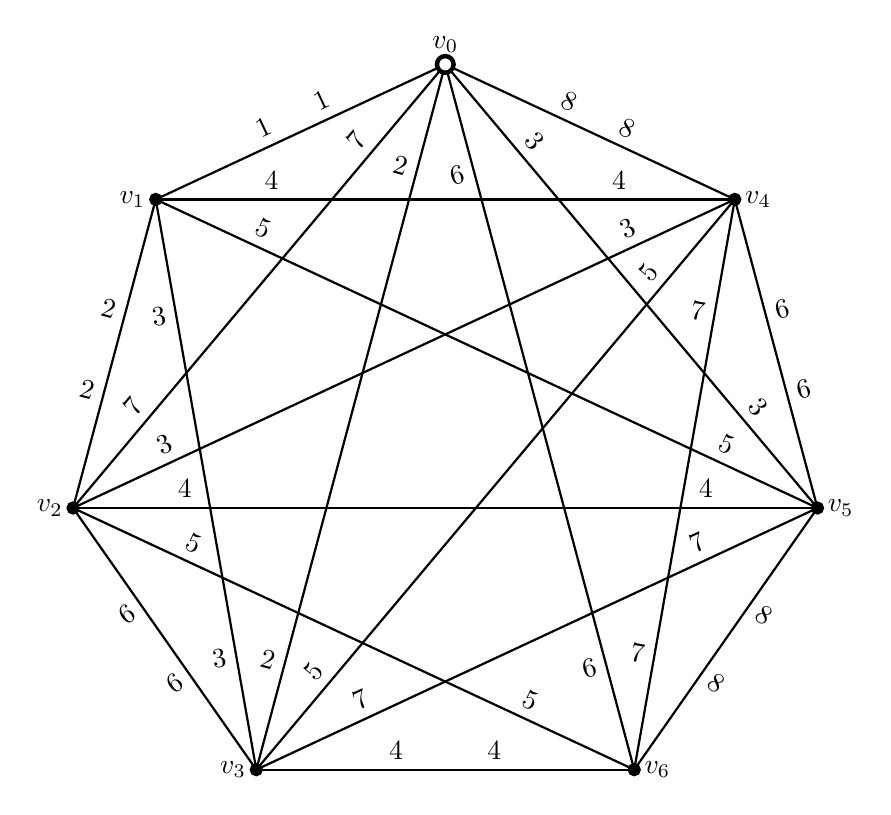
\begin{tikzpicture}[style=thick]
    \coordinate (V3) at (-120:4.8cm);
    \coordinate (V2) at (-170:4.8cm);
    \coordinate (V1) at (140:4.8cm);
    \coordinate (V0) at (90:4.8cm);
    \coordinate (V4) at (40:4.8cm);
    \coordinate (V5) at (-10:4.8cm);
    \coordinate (V6) at (-60:4.8cm);
    
    \draw (V0) -- node [sloped,above,pos=0.4] {$1$} node [sloped,above,pos=0.6] {$1$} (V1);
    \draw (V0) -- node [sloped,above,pos=0.2] {$7$} node [sloped,above,pos=0.8] {$7$} (V2);
    \draw (V0) -- node [sloped,left,rotate=-90,pos=0.15] {$2$} node [sloped,left,rotate=-90,pos=0.85] {$2$} (V3);
    \draw (V0) -- node [sloped,above,pos=0.4] {$8$} node [sloped,above,pos=0.6] {$8$} (V4);
    \draw (V0) -- node [sloped,above,pos=0.2] {$3$} node [sloped,above,pos=0.8] {$3$} (V5);
    \draw (V0) -- node [sloped,left,rotate=90,pos=0.15] {$6$} node [sloped,left,rotate=90,pos=0.85] {$6$} (V6);
    
    \draw (V1) -- node [sloped,left,rotate=-90,pos=0.37] {$2$} node [sloped,left,rotate=-90,pos=0.63] {$2$} (V2);
    \draw (V1) -- node [sloped,left,rotate=90,pos=0.2] {$3$} node [sloped,left,rotate=90,pos=0.8] {$3$} (V3);
    \draw (V1) -- node [sloped,above,pos=0.2] {$4$} node [sloped,above,pos=0.8] {$4$} (V4);
    \draw (V1) -- node [sloped,above,pos=0.15] {$5$} node [sloped,above,pos=0.85] {$5$} (V5);
    % \draw (V1) -- node [sloped,left,rotate=-90] {$0$} (V6);
    
    \draw (V2) -- node [sloped,left,rotate=90,pos=0.37] {$6$} node [sloped,left,rotate=90,pos=0.63] {$6$} (V3);
    \draw (V2) -- node [sloped,above,pos=0.15] {$3$} node [sloped,above,pos=0.85] {$3$} (V4);
    \draw (V2) -- node [sloped,above,pos=0.15] {$4$} node [sloped,above,pos=0.85] {$4$} (V5);
    \draw (V2) -- node [sloped,above,pos=0.2] {$5$} node [sloped,above,pos=0.8] {$5$} (V6);
    
    \draw (V3) -- node [sloped,above,pos=0.15] {$5$} node [sloped,above,pos=0.85] {$5$} (V4);
    \draw (V3) -- node [sloped,above,pos=0.2] {$7$} node [sloped,above,pos=0.8] {$7$} (V5);
    \draw (V3) -- node [sloped,above,pos=0.37] {$4$} node [sloped,above,pos=0.63] {$4$} (V6);
    
    \draw (V4) -- node [sloped,right,rotate=90,pos=0.37] {$6$} node [sloped,right,rotate=90,pos=0.63] {$6$} (V5);
    \draw (V4) -- node [sloped,left,rotate=-90,pos=0.2] {$7$} node [sloped,left,rotate=-90,pos=0.8] {$7$} (V6);
    
    \draw (V5) -- node [sloped,right,rotate=-90,pos=0.37] {$8$} node [sloped,right,rotate=-90,pos=0.63] {$8$} (V6);
    
    \draw[fill=white,style=ultra thick] (V0) circle (3pt) node [above] {$v_0$};
    \draw[fill=black] (V1) circle (2pt) node [left] {$v_1$};
    \draw[fill=black] (V2) circle (2pt) node [left] {$v_2$};
    \draw[fill=black] (V3) circle (2pt) node [left] {$v_3$};
    \draw[fill=black] (V4) circle (2pt) node [right] {$v_4$};
    \draw[fill=black] (V5) circle (2pt) node [right] {$v_5$};
    \draw[fill=black] (V6) circle (2pt) node [right] {$v_6$};
  \end{tikzpicture}
  \end{center}
  \caption{$K_7-e$ գրաֆի $\beta$ ճիշտ կողային ներկումը $8$ գույներով, որտեղ $def( v_0,\beta)=def(K_7-e)=2$:}
  \label{K7-minus-edge}
\end{figure}

\begin{theorem}
\label{t3_wdef_near_complete} Եթե $n\in \mathbb{N}$, ապա
$w_{def}(K_{2n+1}-e)=3n-1$:
\end{theorem}
\begin{proof}[Ապացույց]
Թեորեմ \ref{t3_def_near_complete}-ի ապացույցից ունենք, որ
$K_{2n+1}-e$ գրաֆը ունի $\alpha$ ճիշտ կողային ներկում $(3n-1)$ գույներով և $def(K_{2n+1}-e,\alpha)=def(K_{2n+1}-e)=n-1$ դեֆիցիտով: Այստեղից հետևում է, որ $w_{def}(K_{2n+1}-e)\leq 3n-1$: Մյուս կողմից, քանի որ $K_{2n+1}-e$ գրաֆը չունի կատարյալ զուգակցում, $\delta(K_{2n+1}-e)=2n-1$ և $def(K_{2n+1}-e)=n-1$, Թեորեմ
\ref{t3_wdef_nopm}-ի համաձայն ստանում ենք, որ $w_{def}(K_{2n+1}-e)\geq
2(2n-1)-n+1=3n-1$:
\end{proof}

\begin{theorem}
\label{t3_def_K1mn} Կամայական $m,n\in \mathbb{N}$ թվերի համար
\begin{center}
$def\left(K_{1,m,n}\right)=\left\{
\begin{tabular}{ll}
$0$, & երբ $(m+1,n+1)=1$,\\
$1$, & հակառակ դեպքում:\\
\end{tabular}%
\right.$
\end{center}
\end{theorem}
\begin{proof}[Ապացույց] Ըստ Թեորեմներ \ref{t1_K1mn_coprime}-ի և \ref{t1_K1mn_nocoprime}-ի, $K_{1,m,n}\in \mathfrak{N}$ այն և միայն դեպքում, երբ
$(m+1,n+1)=1$ կամայական $m,n\in \mathbb{N}$ թվերի համար: Այստեղից հետևում է, որ
$def\left(K_{1,m,n}\right)=0$, երբ $(m+1,n+1)=1$, և
$def\left(K_{1,m,n}\right)\geq 1$, երբ $(m+1,n+1)>1$: Այժմ ցույց տանք, որ $def\left(K_{1,m,n}\right)\leq 1$: Դիցուք.
\begin{align*}
V\left(K_{1,m,n}\right)&=\{u_{1},\ldots,u_{m},v_{1},\ldots,v_{n},w\}\\
E\left(K_{1,m,n}\right)&=\left\{u_{i}v_{j}\colon\,1\leq i\leq
m,1\leq j\leq n\right\}\cup \{wu_{i}\colon\,1\leq i\leq m\}\cup
\{wv_{j}\colon\,1\leq j\leq n\}:
\end{align*}
Սահմանենք $K_{1,m,n}$-ի $\alpha$ կողային ներկումը հետևյալ կերպ.

\begin{description}
\item[(1)] երբ $1\leq i\leq m$ և $1\leq j\leq n$, 
$\alpha\left(u_{i}v_{j}\right)=i+j$,

\item[(2)] երբ $1\leq i\leq m$, $\alpha\left(wu_{i}\right)=i$,

\item[(3)] երբ $1\leq j\leq n$, $\alpha\left(wv_{j}\right)=m+1+j$:
\end{description} % արժի շուռ տալ

Ապացուցենք, որ $\alpha$-ն $K_{1,m,n}$-ի ճիշտ կողային ներկում է $m+n+1$ գույներով և  $def\left(K_{1,m,n},\alpha\right)=1$ դեֆիցիտով: Ըստ $\alpha$-ի սահմանման ունենք, որ
\begin{description}
\item[1)] երբ $1\leq i\leq m$,

$S\left(u_{i},\alpha\right)=[i+1,n+i]\cup \{i\}=[i,n+i]$ համաձայն (1)-ի և (2)-ի,

\item[2)] երբ $1\leq j\leq n$,

$S\left(v_{j},\alpha\right)=[j+1,m+j]\cup \{m+1+j\}=[j+1,m+1+j]$ համաձայն (1)-ի և (3)-ի,

\item[3)] $S\left(w,\alpha\right)=[1,m]\cup [m+2,m+n+1]$
համաձայն (2)-ի և (3)-ի:
\end{description} % արժի շուռ տալ

Այստեղից հետևում է, որ $\alpha$-ն $K_{1,m,n}$-ի ճիշտ կողային ներկում է $m+n+1$ գույներով և $def\left(K_{1,m,n},\alpha\right)=1$ դեֆիցիտով
($m,n\in \mathbb{N}$), ուստի $def\left(K_{1,m,n}\right)\leq 1$ երբ
$(m+1,n+1)>1$:
\end{proof}
\end{hide}